\documentclass[11pt,a4paper]{article}
\usepackage[top=2.8cm,bottom=2.4cm,left=2.4cm,right=2.4cm,a4paper,twoside]{geometry}
\usepackage{amssymb,amsmath}% Equations
\usepackage[title,titletoc,toc]{appendix}% Appendix
%\usepackage{hyperref}
\usepackage{graphicx,color,psfrag}% Graphics, Figures
\usepackage{fancyhdr}
\usepackage{longtable,tabularx}
\usepackage{multirow}
\usepackage{multicol}% to allow multiple columns
\usepackage[no-math]{fontspec}
\usepackage{xunicode}
\usepackage{xltxtra}
\usepackage{sectsty}% to customize setting in section heads
\usepackage{wrapfig}
\usepackage{indentfirst}

\newenvironment{Figure}
  {\par\medskip\noindent\minipage{\linewidth}}
  {\endminipage\par\medskip}

\newenvironment{Table}
   {\par\bigskip\noindent\minipage{\columnwidth}\centering}
   {\endminipage\par\bigskip}

\usepackage{secdot} % add a period after section numbers.
\sectiondot{subsection} %add a period after subsection numbers. 
\sectiondot{subsubsection} %add a period after subsubsection numbers.

\usepackage[justification=RaggedRight,singlelinecheck=false]{caption}% to change the table caption left-justified.
%\usepackage[font=small,labelfont=bf, justification=justified, format=plain]{caption}
%\usepackage[justification=justified, format=plain]{caption}
%\usepackage{caption}
%\captionsetup{justification=raggedright,singlelinecheck=false}
\captionsetup[figure]{labelsep=period}% to create a period . after Figure name.		
\captionsetup[table]{labelsep=period}% to create a period . after Table name.		

\setcounter{page}{101} % set the starting page number 

\sectionfont{\fontsize{12}{15}\selectfont}% adjust the section font size to 12pt
\subsectionfont{\fontsize{11}{13}\selectfont}% adjust the subsection font size to 11pt


\defaultfontfeatures{Scale=1.0,Mapping=tex-text}
\setmainfont[Scale=1.0]{GaramondNo8}

%\pagestyle{fancy}
%\fancyhead{}% clear all header fields
%\fancyhead[RO,LE]{\footnotesize DOI:10.4186/ej.year.vol.issue.pp}
%\fancyfoot{}% clear all footer fields
%\fancyfoot[LE]{\footnotesize \thepage \hfill ENGINEERING JOURNAL Volume \# Issue \#, ISSN 0125-8281 (http://www.engj.org/)}
%\fancyfoot[RO]{\footnotesize ENGINEERING JOURNAL Volume \# Issue \#, ISSN 0125-8281 (http://www.engj.org/) \hfill \thepage}

\renewcommand{\headrulewidth}{0pt}
\renewcommand{\figurename}{Fig.}

\begin{document}
\thispagestyle{empty}
\begin{center}

\includegraphics[width=1\linewidth]{ej_banner.png}
\end{center}
\vspace{5mm}

\begin{flushleft}
\textit{\fontsize{14}{17}\selectfont Article/Review} \\ [4ex]
\textbf{\fontsize{20}{24}\selectfont \LaTeX~Template for Engineering Journal} \\ [5ex]
\textbf{\fontsize{12}{15}\selectfont First Author{\normalfont{\textsuperscript{1,a}}}, Second Author{\normalfont{\textsuperscript{1,b,*}}}, and Third Author{\normalfont{\textsuperscript{2}}}} \\ [2ex]
{\fontsize{8}{12}\selectfont 1} First and Second Authors’ affiliation and address \\
{\fontsize{8}{12}\selectfont 2} Third Author’s affiliation and address \\
E-mail: {\textsuperscript{a}}first.author@email.com, {\textsuperscript{b}}second.author@email.com (Corresponding author) \\ [5ex]
\end{flushleft}

%--------------------------ABSTRACT-------------------------------------
{\paragraph{Abstract.} An abstract is a shortened version of the paper and should contain all information necessary for the reader to determine: (1) what the objectives of the study were; (2) how the study was done; (3) what results were obtained; (4) the significance of the results. The typical length of an abstract is 150 – 200 words.}
%---------------------------------------------------------------------------


{\flushleft \textbf{Keywords:} Keyword1, keyword2, keyword3, etc.}

\vfill
\begin{flushleft}
\textbf{ENGINEERING JOURNAL} Volume \# Issue \# \\
Received Date Month Year \\
Accepted Date Month Year \\
Published Date Month Year \\
Online at http://www.engj.org/ \\
DOI:10.4186/ej.20xx.xx.x.xx
\end{flushleft}

\newpage


\newgeometry{top=1.95cm,bottom=1.8cm,left=1.6cm,right=1.6cm,headsep=0.5cm,a4paper,twoside}

\pagestyle{fancy}
\fancyhead{}% clear all header fields
\fancyhead[RO,LE]{\footnotesize DOI:10.4186/ej.year.vol.issue.pp}
\fancyfoot{}% clear all footer fields
\fancyfoot[LE]{\footnotesize \thepage \hfill ENGINEERING JOURNAL Volume \# Issue \#, ISSN 0125-8281 (http://www.engj.org/)}
\fancyfoot[RO]{\footnotesize ENGINEERING JOURNAL Volume \# Issue \#, ISSN 0125-8281 (http://www.engj.org/) \hfill \thepage}

\begin{multicols}{2}

%-----------------------------------------------Introduction-------------------------------------------------------


\section{Introduction}
We request authors to follow this guideline and format their manuscripts exactly the same as this document. The easiest way to do this is download this template and replace its contents with those in your manuscript.


\section{Page Dimensions}
All material on all pages should fit within an area of A4 (21 $\times$ 29.7 cm), 2.8 cm from the top of the page and ending with 2.4 cm from the bottom. The left and right margins should both be 2.4 cm.

\section{Main Text}
This section provides details for typesetting your manuscript according to the formatting guidelines set for Engineering Journal. Use 11-point Garamond regular font for typesetting of the main text in the document.

The main text starts at the top of the page and continues in one column format. Place an indentation for each paragraph starting from the second in all sections or subsections. There is no space between paragraphs within the text. Add an 11-point space at both before and after the text in each section or subsection.

\subsection{Default Fonts}
Use only Garamond fonts throughout the document. If any special font is required to display the text properly, please mention this during the manuscript submission process.

\subsection{Typeset Text}
Use 20-point-bold Garamond font for the paper title. Author’s names (12-point Garamond bold) and affiliations (11-point Garamond regular) are aligned left. Separate addresses for different affiliations and add a space between authors’ names and affiliations.

\subsection{Page Numbering / Header and Footer}
Do not include headers, footers, or page numbers other than those already set in this manuscript. Note that the headers, footers or page numbers are different for the first page and the rest of the pages. Actual page numbers and other running heads will be modified when publications are assembled.

\subsection{Mathematics}
Math typesetting can be done by Equation Editor, or by any other system that produce clear math types (Garamond or Time New Roman regular 11 pt.). Symbols and shorter expression can be placed within the text, e.g. ε→0.  More complex expression should be placed in a center of a new line:
\begin{equation}
E = mc^2
\end{equation}


\begin{Figure}
	\begin{center}
		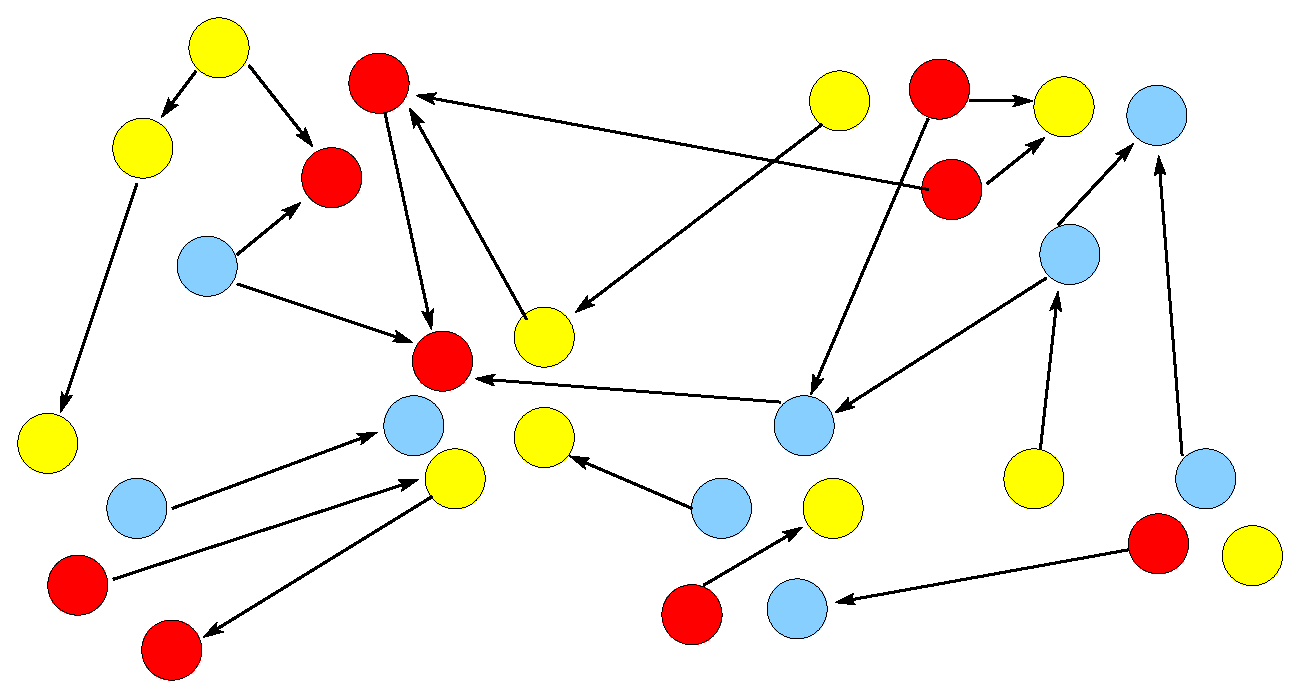
\includegraphics[width=5cm]{gm.eps}
	\end{center}
	\captionof{figure}{If you want your figure to fit into one of the two columns, you must use the Figure environment (with a captical F).}
\end{Figure}


\begin{Table}
	\begin{tabular}{|c|c|} \hline
This & is \\ \hline
a & test \\ \hline
	\end{tabular} 
	\captionof{table}{If you want your table to fit into a single column, you must use the Table environment (with a capital T).}
\end{Table}


All equations should be numbered, right justified. They should be referred just like figures and tables, e.g. Eq. (1). Unless it is absolutely necessary, equation numbers should not have part to them, e.g. instead of using Eq. 1(a) and Eq. 1(b). Number them as Eq. (1) and Eq. (2).

\section{Figures/Captions}
Place tables/figures/images in text as close to the reference as possible (see figure 1). Each figure or table must include a caption set in 11-point Garamond regular font, placed below the figure or table. The caption is left justified.

\begin{figure*}[ht]
	\begin{center}
		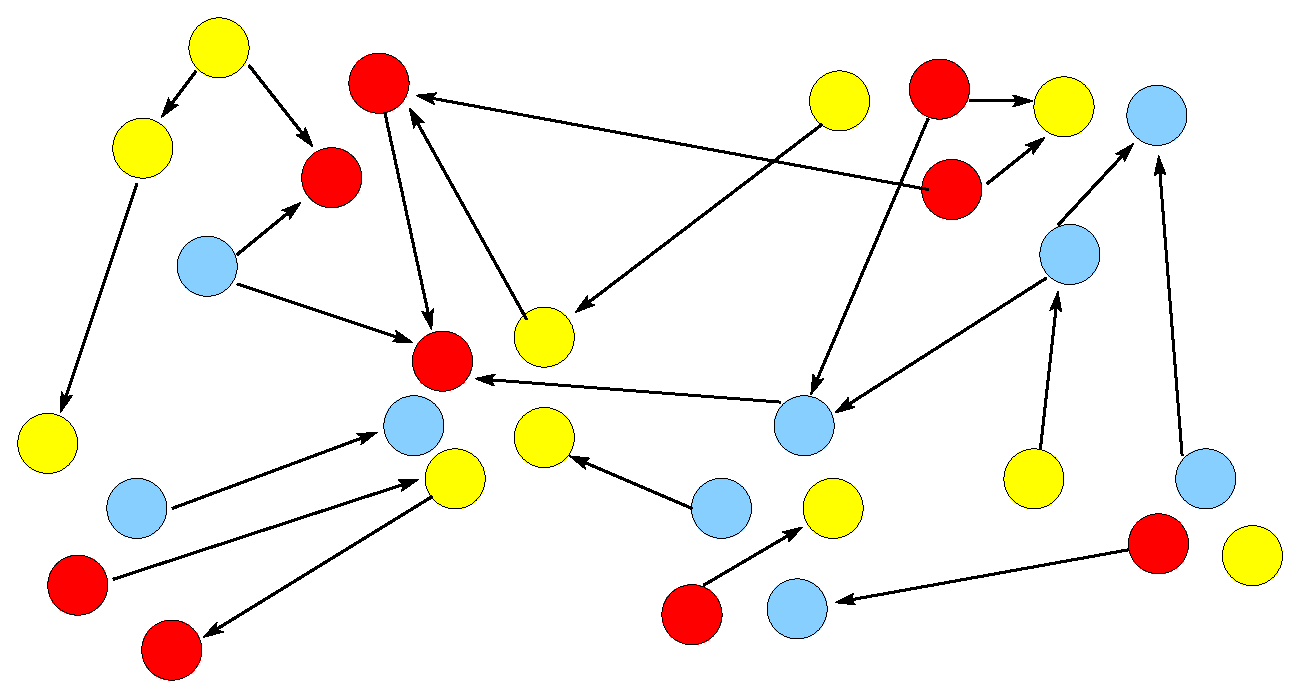
\includegraphics[width=0.7\linewidth]{gm.eps}
	\end{center}
	\caption{If your figure should span the entire page, use this environment instead.}
\end{figure*}

\begin{table*}[ht]
\caption{Font type and size list for EJ's template.}
\centering
\begin{tabular}{|l|c|c|r|} \hline
Item & Font & Font Type & Font Size \\ \hline
Title & Garamond & Bold & 20 \\
Author names & Garamond & Bold & 12 \\
Author affiliation/email & Garamond & Regular & 11 \\
Abstract/Keywords & Garamond & Regular & 11 \\
Level 1 headings & Garamond & Bold & 12 \\
Level 2 headings & Garamond & Bold & 11 \\
Level 3 headings & Garamond & Regular & 11 \\
Figure/table captions & Garamond & Regular & 11 \\
Main text/References & Garamond & Regular & 11 \\ \hline
\end{tabular}
\end{table*}





Reference to the figure should follow the format “Fig. 1”. Use “Figure 1” instead if it is at the beginning of a sentence. Figure numbering and referencing should be done sequentially, e.g. Fig. 1, Fig. 2, Table 1, Table 2., etc. Use Fig. 1(a), Fig. 1(b), etc. for figures with multiple parts.

\section{Sections}
The heading of sections should be in 12-point Garamond bold font and flush left. Sections and subsequent sub-sections should be numbered and flush left in the same manner. Sections numbers are in Roman style.

\subsection{Subsection Level 1}
Use 11-point Garamond bold font for the heading of subsections.

\subsubsection{Sub-subsection Level 2}
Use 11-point Garamond regular font for the heading of subsubsections.

\section{About References}
References should be arranged by the order in which they appear in the text. Only the references that are cited in the text should be added to the reference list. Authors should follow the format as follows:

\nocite{StR:12}
\nocite{PMB:09}
\nocite{RuS:10}

%--------------------------------------Reference---------------------------------------------------------
\newcommand{\BIBdecl}{\setlength{\itemsep}{-0.3em}}
\bibliographystyle{IEEEtran}
\bibliography{ref}

\end{multicols}

\begin{center}

\includegraphics[width=4.76cm,height=0.18cm]{h-bar.png}
\end{center}

\newpage

\begin{wrapfigure}{l}{3cm}
    
\includegraphics[width=2.54cm,height=3.4cm]{author-01.png}
\end{wrapfigure}


\noindent \textbf{First A. Author} and all authors may include biographies. The first paragraph may contain a place and/or date of birth (list place, then date). Next, the author’s educational background is listed. The degrees should be listed with type of degree in what field, which institution, city, state, and country, and year the degree was earned. The author’s major field of study should be lower-cased. The second paragraph uses the pronoun of the person (he or she) and not the author’s last name. It lists work experience. Information concerning previous publications may be included. The third paragraph begins with the author’s title and last name (e.g., Dr. Smith, Prof. Jones, Mr. Kajor, Ms. Hunter). List any memberships in professional societies. Finally, list any awards received. If a photograph is provided, it should be of good quality, and professional-looking. Below is an example of an author’s biography. \\

%\newpage

\begin{wrapfigure}{l}{3cm}
    
\includegraphics[width=2.54cm,height=3.4cm]{author-02.png}
\end{wrapfigure}

\noindent \textbf{Second B. Author} was born in Greenwich Village, New York, NY, USA in 1977. She received the B.S. and M.S. degrees in aerospace engineering from the University of Virginia, Charlottesville, in 2001 and the Ph.D. degree in mechanical engineering from Drexel University, Philadelphia, PA, in 2008. From 2001 to 2004, she was a Research Assistant with the Princeton Plasma Physics Laboratory. Since 2009, she has been an Assistant Professor with the Mechanical Engineering Department, Texas A\&M University, College Station. She is the author of three books, more than 150 articles, and more than 70 inventions. Her research interests include high-pressure and high-density nonthermal plasma discharge processes and applications, microscale plasma discharges, discharges in liquids, spectroscopic diagnostics, plasma propulsion, and innovation plasma applications. She is an Associate Editor of the journal Earth, Moon, Planets, and holds two patents. Dr. Author was a recipient of the International Association of Geomagnetism and Aeronomy Young Scientist Award for Excellence in 2008, and the IEEE Electromagnetic Compatibility Society Best Symposium Paper Award in 2011.



\end{document}
